\documentclass[
  % all of the below options are optional and can be left out
  % course name (default: 2IL50 Data Structures)
  course = {{16-720B Computer Vision}},
  % quartile (default: 3)
  quartile = {{1}},
  % assignment number/name (default: 1)
  assignment = 3-Neural\ Networks\ for\ Recognition,
  % student name (default: Some One)
  name = {{Kangle Deng}},
  % student number, NOT S-number (default: 0123456)
  % studentnumber = {{0123456 ; 0314159}},
  % student email (default: s.one@student.tue.nl)
  email = {{kangled@andrew.cmu.edu}},
  % first exercise number (default: 1)
  firstexercise = 1
]{aga-homework}

\usepackage{url}
\usepackage{subfigure}

\begin{document}
\section{Theory}
\noindent \textbf{Q1.1} 

Let $y = x + c$. Then for each index $i$, we have:
\begin{equation*}
\begin{aligned}
    softmax(y_i) & = \frac{e^{y_i}}{\sum_j e^{y_j}} \\
    & = \frac{e^{x_i + c}}{\sum_j e^{x_j + c}} \\
    & = \frac{e^c \cdot e^{x_i}}{e^c \cdot \sum_j e^{x_j}} \\
    & =  \frac{e^{x_i}}{\sum_j e^{x_j}} \\
    & = softmax(x_i).
\end{aligned}
\end{equation*}

When $c = 0$, both the numerator and denominator can be very large, this leads to the risk of overflow. When $c = -\max x_i$, all the numerators are less than or equal to $1$, and the denominator also has an upper bound of $n$, where $n$ is number of channels.

\noindent \textbf{Q1.2}

\begin{itemize}
    \item The range of each element is $[0,1]$. The sum over all elements is 1.
    \item Softmax takes an arbitrary real valued vector $x$ and turns it into a \textbf{discrete probability distribution}.
    \item The first step is calculating the weight for each element. The second step is summing over all the weights. The third step is calculating each element using its own weight and the total weight.
\end{itemize}

\noindent \textbf{Q1.3}
We first state that all the convolutional layers can be seen as fully connected layers $y = Wx + b$, with some redundant information in $W$. Also, a linear activation function can be seen as a fully connected layer.

So a multi-layer neural network without a non-linear activation function can be seen as a series of fully connected layers. We now show that 2 successive fully connected layer $y = W_ix + b_i$ and $y = W_jx+b_j$ can be expressed as one fully connected layer:

\begin{equation*}
    y = W_j(W_ix + b_i) + b_j = W_jW_ix + (W_jb_i + b_j).
\end{equation*}

From mathematical induction, we show that multi-layer neural networks without a non-linear activation function are equivalent to a single fully connected layer, which is also known as linear regression.

\noindent \textbf{Q1.4}
\begin{equation*}
    \sigma'(x) = -\frac{1}{(1+e^{-x})^2}(-e^{-x}) = \frac{e^{-x}}{(1+e^{-x})^2}
\end{equation*}

Note that $e^{-x} = \frac{1}{\sigma(x)} - 1$, we have $\sigma'(x) = \frac{\frac{1}{\sigma(x)} - 1}{\frac{1}{\sigma^2(x)}} = \sigma(x) - \sigma^2(x)$.

\noindent \textbf{Q1.5}

To solve $\frac{\partial J}{\partial W}$, we consider:
\begin{equation*}
    \begin{aligned}
        % \frac{\partial J}{\partial W} & = \frac{\partial J}{\partial y} \cdot \frac{\partial y}{\partial W} = \delta \cdot x^T. \\
        & dJ = \frac{\partial J}{\partial y}^T \cdot dy = \frac{\partial J}{\partial y}^T \cdot dW \cdot x = tr(\frac{\partial J}{\partial y}^T \cdot dW \cdot x) = tr(x \cdot \frac{\partial J}{\partial y}^T \cdot dW) = tr((\frac{\partial J}{\partial y} \cdot x^T)^T \cdot dW). \\
    \end{aligned}
\end{equation*}
So we have $ \frac{\partial J}{\partial W} = \frac{\partial J}{\partial y} \cdot x^T = \delta \cdot x^T.$

To solve $\frac{\partial J}{\partial x}$, we consider:
\begin{equation*}
    dJ = \frac{\partial J}{\partial y}^T \cdot dy = \frac{\partial J}{\partial y}^T \cdot W \cdot dx = (W^T \cdot \frac{\partial J}{\partial y})^T \cdot dx.
\end{equation*}
So we have $\frac{\partial J}{\partial x} = W^T \cdot \frac{\partial J}{\partial y} = W^T \cdot \delta$.

To solve $\frac{\partial J}{\partial b}$, we consider:
\begin{equation*}
    dJ = \frac{\partial J}{\partial y}^T \cdot dy = \frac{\partial J}{\partial y}^T \cdot \frac{dy}{db} \cdot db = \frac{\partial J}{\partial y}^T \cdot db.
\end{equation*}
So, $\frac{\partial J}{\partial b} = \frac{\partial J}{\partial y} = \delta$.

\noindent \textbf{Q1.6}

Note that

\begin{equation*}
    y_{d,i,j} = \sum \limits_{c=0}^{C-1} \sum \limits_{w=0}^{K-1} \sum \limits_{h=0}^{K-1} W_{d,c,w,h} x_{c,i+w,j+h} + b_d.
\end{equation*}

So,
\begin{equation*}
\begin{aligned}
        \frac{\partial J}{\partial W_{d_0,c_0,w_0,h_0}} & = \sum \limits_{d=0}^{D-1} \sum \limits_{i=0}^{M_O-1} \sum \limits_{j=0}^{N_O-1} \frac{\partial J}{\partial y_{d,i,j}} \cdot \frac{\partial y_{d,i,j}}{\partial W_{d_0,c_0,w_0,h_0}} \\
        & = \sum \limits_{i=0}^{M_O-1} \sum \limits_{j=0}^{N_O-1} \frac{\partial J}{\partial y_{d_0,i,j}} \cdot \frac{\partial y_{d_0,i,j}}{\partial W_{d_0,c_0,w_0,h_0}} \\
        & = \sum \limits_{i=0}^{M_O-1} \sum \limits_{j=0}^{N_O-1} \delta_{d_0,i,j} \cdot \sum \limits_{c=0}^{C-1} x_{c,i+w_0,j+h_0} \\
        & =\sum \limits_{c=0}^{C-1} \sum \limits_{i=0}^{M_O-1} \sum \limits_{j=0}^{N_O-1} \delta_{d_0,i,j} \cdot  x_{c,i+w_0,j+h_0}.
\end{aligned}
\end{equation*}

\begin{equation*}
    \begin{aligned}
         \frac{\partial J}{\partial x_{c_0,i_0,j_0}} & =   \sum \limits_{d=0}^{D-1} \sum \limits_{i=0}^{M_O-1} \sum \limits_{j=0}^{N_O-1} \frac{\partial J}{\partial y_{d,i,j}} \cdot \frac{\partial y_{d,i,j}}{\partial x_{c_0,i_0,j_0}} \\
         & =   \sum \limits_{d=0}^{D-1} \sum \limits_{i=\max(i_0-K+1,0)}^{\min(i_0,M_O)} \sum \limits_{j=\max(j_0-K+ 1,0)}^{\min(j_0,N_O)} \frac{\partial J}{\partial y_{d,i,j}} \cdot \frac{\partial y_{d,i,j}}{\partial x_{c_0,i_0,j_0}} \\
         & = \sum \limits_{d=0}^{D-1} \sum \limits_{i=\max(i_0-K+1,0)}^{\min(i_0,M_O)} \sum \limits_{j=\max(j_0-K+ 1,0)}^{\min(j_0,N_O)} \delta_{d,i,j} \cdot W_{d,c_0,i_0-i,j_0-j} \\
         & = \sum \limits_{d=0}^{D-1} \sum \limits_{w=\max(0,i_0-M_O)}^{\min(K-1,i_0)} \sum \limits_{h=\max(0,j_0-N_O)}^{\min(K-1,j_0)} \delta_{d,i,j} \cdot W_{d,c_0,w,h}.
    \end{aligned}
\end{equation*}

\begin{equation*}
    \begin{aligned}
        \frac{\partial J}{\partial b_{d_0}} & = \sum \limits_{d=0}^{D-1} \sum \limits_{i=0}^{M_O-1} \sum \limits_{j=0}^{N_O-1} \frac{\partial J}{\partial y_{d,i,j}} \cdot \frac{\partial y_{d,i,j}}{\partial b_{d_0}} = \sum \limits_{i=0}^{M_O-1} \sum \limits_{j=0}^{N_O-1} \frac{\partial J}{\partial y_{d_0,i,j}} \cdot \frac{\partial y_{d_0,i,j}}{\partial b_{d_0}} = \sum \limits_{i=0}^{M_O-1} \sum \limits_{j=0}^{N_O-1} \delta_{d_0,i,j}.
    \end{aligned}
\end{equation*}
% To solve $\frac{\partial J}{\partial W}$, we consider:
% \begin{equation*}
%     \begin{aligned}
%         dJ = \frac{\partial J}{\partial y}^T \cdot dy = \frac{\partial J}{\partial y}^T \cdot (dW * x)_{D\times M_O \times N_O} = . 
%     \end{aligned}
% \end{equation*}

\noindent \textbf{Q1.7}

\begin{enumerate}
    \item Note that $\sigma'(x) = \sigma(x) - \sigma^2(x) = -(\sigma(x)-\frac{1}{2})^2+\frac{1}{4}$, and $\sigma(x) \in [0, 1]$. So $\sigma'(x) \in [0, \frac{1}{4}]$. Every time the back-propagation algorithm passes through a sigmoid layer, it will multiply $\sigma'()$ to the gradient, which is a scaling factor ranging in $[0,\frac{1}{4}]$. %Even worse, when $\sigma(x)$ is close to $0$, $\sigma'(x)$ is also close to 0, which means when the gradient is close to 0, it will be even closer to $0$ when passing through the sigmoid layer. 
    So if there are many sigmoid layers, the gradient will be close to $0$.
    \item $\tanh{(x)} = \frac{-(1+e^{-2x})+2}{1+e^{-2x}} = -1 + \frac{2}{1+e^{-2x}} \in [0, 2]$. And the output range of sigmoid is $[0,1]$. We might prefer $\tanh$ because the mean value of the output range of $\tanh$ is 0 while the output of sigmoid is always positive. An always positive output will cause the gradients of this layer to be all positive or all negative, which might lead to ``zigzag'' phenomenon during optimization.
    % \item When $\tanh(x)$ is close to $0$, $\tanh'(x)$ is close to $1$. So the ``vanishing gradient'' problem is alleviated.
    \item Note that $\tanh'(x) = 1 - \tanh^2(x)$. When $\tanh(x)$ is close to $0$, $\tanh'(x)$ is close to $1$. If activation values form a good distribution such as Gaussian, they will appear more often around $0$, which makes $\tanh'(x)$ close to $1$. So the ``vanishing gradient'' problem is alleviated.
    \item $\tanh(x) = \frac{-(1+e^{-2x})+2}{1+e^{-2x}} = -1 + \frac{2}{1+e^{-2x}} = 2\sigma(x) - 1$.
\end{enumerate}

\section{Implement a Fully Connected Network}
\subsection{Network Initialization}
\noindent\textbf{Q2.1.1} 

If all the weights and biases are initialized with zeros, all the neurons in the same layer would have the same output, and thus have the same gradients. This would make the weights and biases in a layer always the same, even after training and updating. The network would perform like there's only one neuron in each layer.

\noindent \textbf{Q2.1.3}

As I mentioned in \textbf{Q2.1.1}, we don't want the network to be initialized with same values. So we prefer random numbers. On the other hand, from Fig 6 in the paper, we can see that if we just use the standard initialization, activation values gathers to $0$ rapidly in deeper layers. While those values still keeps good distribution with constant variances if we use Xavier initialization. This helps the optimization a lot during training.

% \subsection{Forward Propagation}

\section{Training Models}
\noindent \textbf{Q3.1.1}

Fig. \ref{fig:cv_hw3_q311} is the plot of the accuracy and loss during training. The final averaged accuracy on the validation set is $76.8\%$. The batch size is set as $32$, and the learning rate is set as $5e-3$.

\begin{figure}
    \centering
    \subfigure[Accuracy]{
    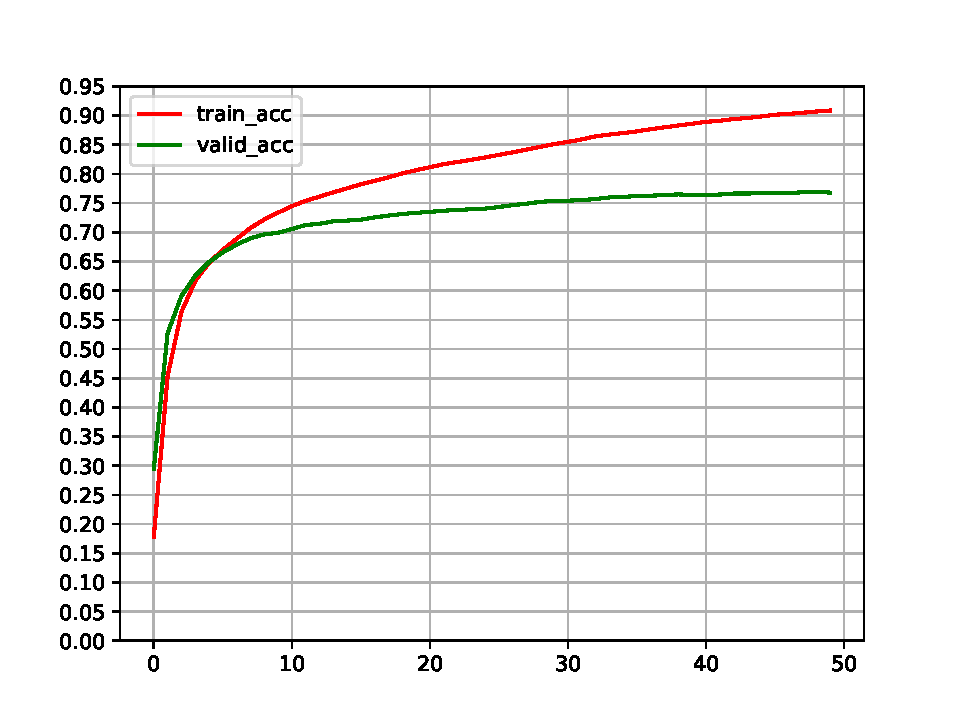
\includegraphics[width=.48\textwidth]{CV/fig/hw3/q3_acc.pdf}}
    \subfigure[Averaged Cross-Entropy Loss]{
    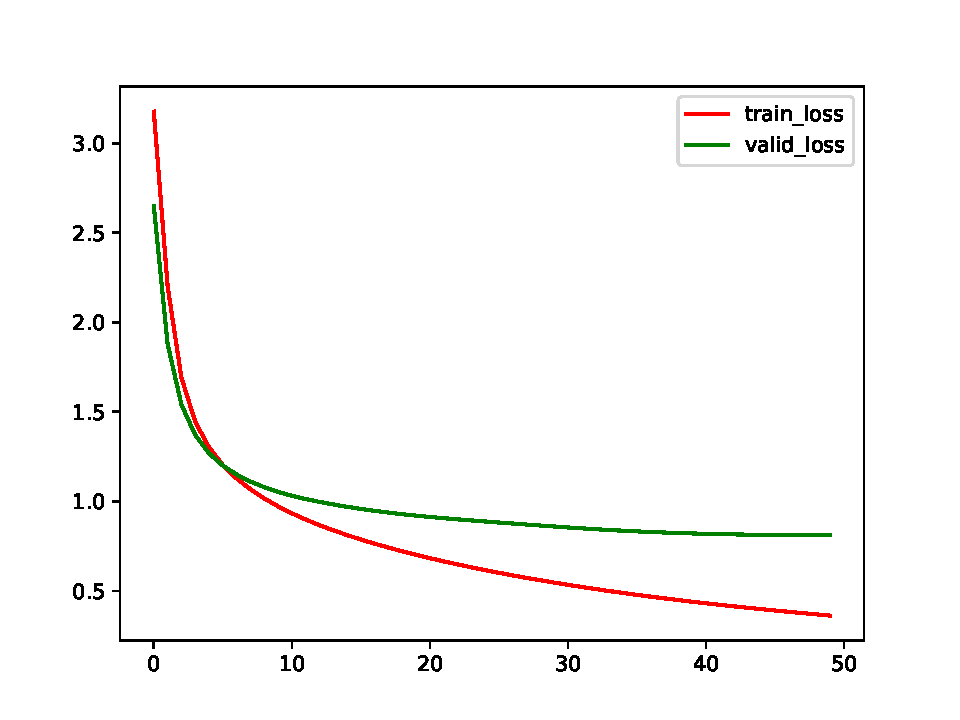
\includegraphics[width=.48\textwidth]{CV/fig/hw3/q3_loss.pdf}}
    \caption{Q3.1.1}
    \label{fig:cv_hw3_q311}
\end{figure}

\noindent \textbf{Q3.1.2}

Fig. \ref{fig:cv_hw3_q312} is the result. I set the learning rate as $5e-4, 5e-3, \text{and} 5e-2$ respectively. When the learning rate is $5e-4$, the optimization step is too small so that the loss does not reach minimum after 50 epoches. When the learning rate is $5e-2$, the optimization step is too large, so it causes the oscillation of the loss. When the learning rate is $5e-3$, it is appropriate so that the model reaches the optimal in a moderate speed. The final accuracy on the test set is $77.9\%$.

\begin{figure}
    \centering
    \subfigure[Accuracy (lr=5e-4)]{
    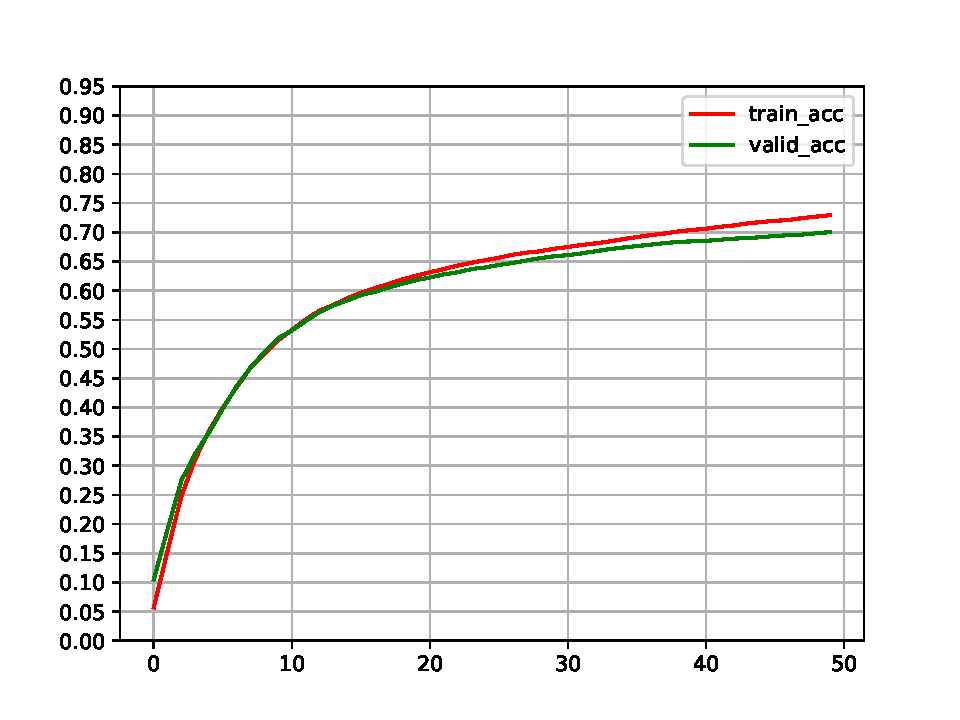
\includegraphics[width=.48\textwidth]{CV/fig/hw3/q312_acc_1.pdf}}
    \subfigure[Averaged Cross-Entropy Loss (lr=5e-4)]{
    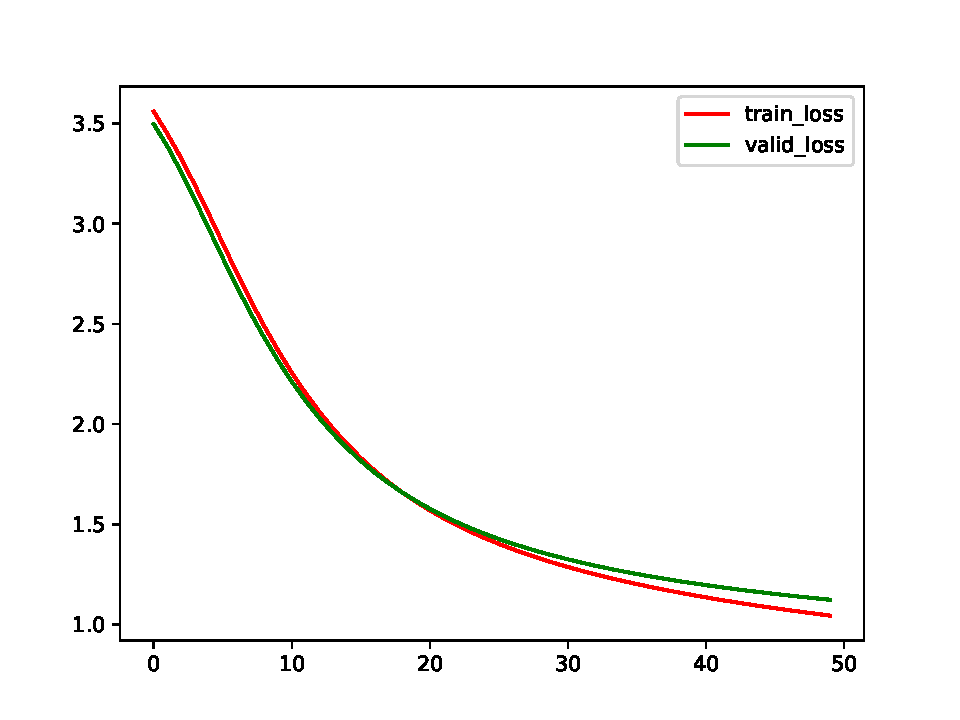
\includegraphics[width=.48\textwidth]{CV/fig/hw3/q312_loss_1.pdf}}
    \subfigure[Accuracy (lr=5e-3)]{
    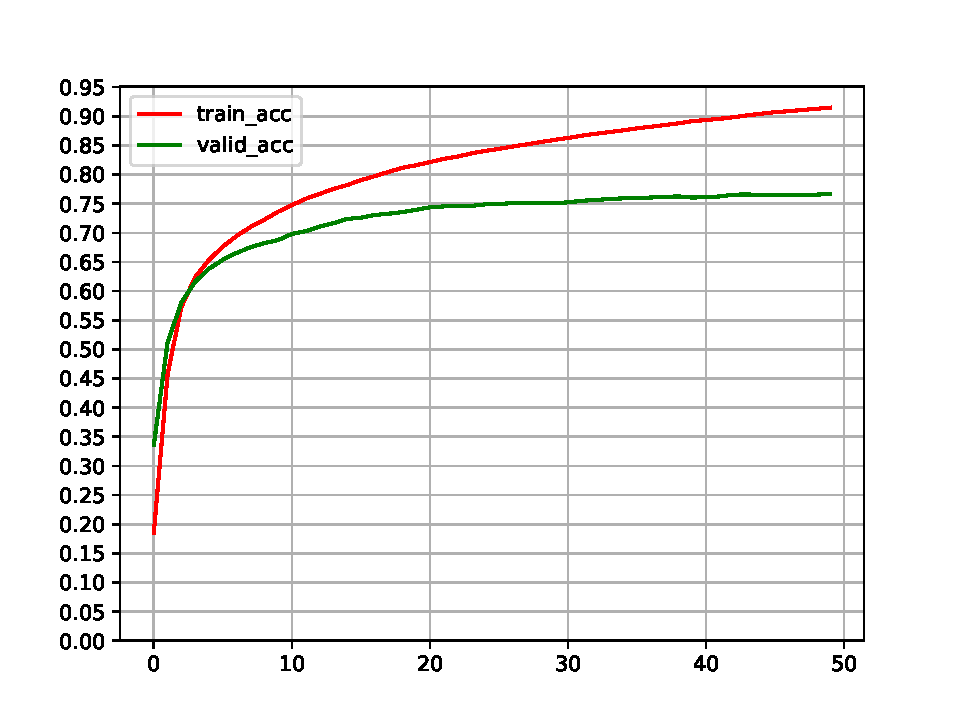
\includegraphics[width=.48\textwidth]{CV/fig/hw3/q312_acc_2.pdf}}
    \subfigure[Averaged Cross-Entropy Loss (lr=5e-3)]{
    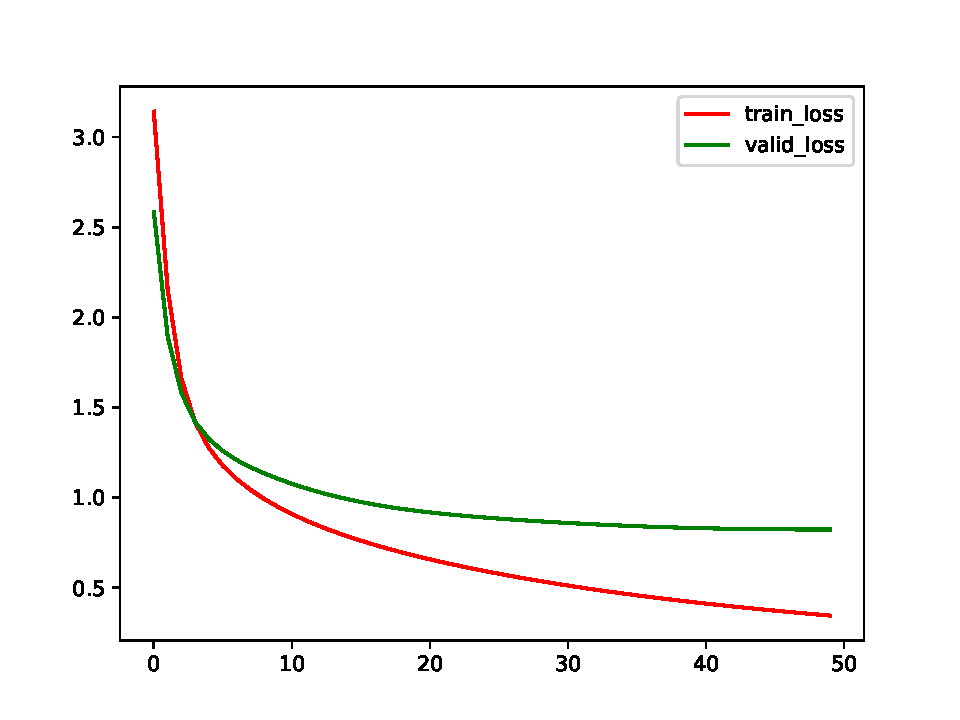
\includegraphics[width=.48\textwidth]{CV/fig/hw3/q312_loss_2.pdf}}
    \subfigure[Accuracy (lr=5e-2)]{
    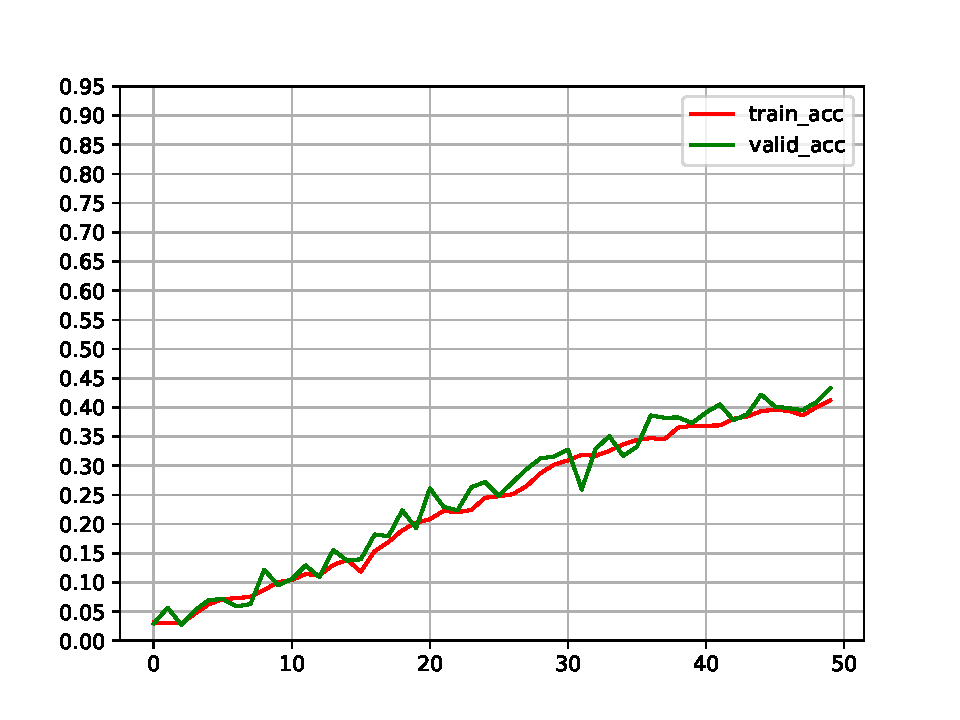
\includegraphics[width=.48\textwidth]{CV/fig/hw3/q312_acc_3.pdf}}
    \subfigure[Averaged Cross-Entropy Loss  (lr=5e-2)]{
    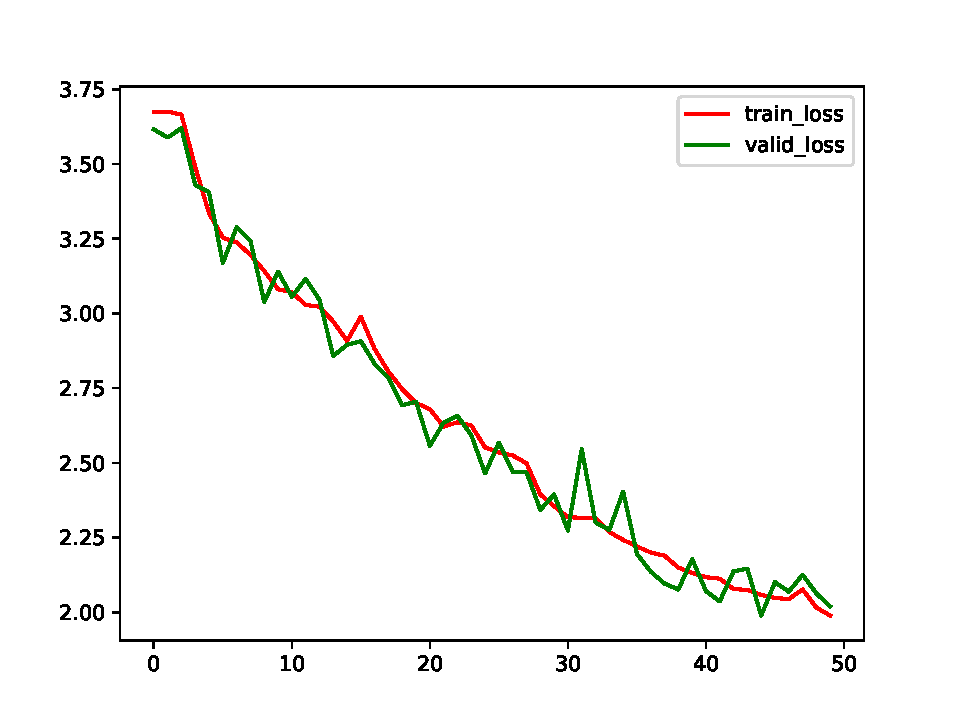
\includegraphics[width=.48\textwidth]{CV/fig/hw3/q312_loss_3.pdf}}
    \caption{Q3.1.2}
    \label{fig:cv_hw3_q312}
\end{figure}

\noindent\textbf{Q3.1.3}

Fig. \ref{fig:cv_hw3_q313} is the result. The initialized weights seem like meaningless noise, while learned weights have some patterns. For example, there're some neurons (7th row 6th column) where low activation appears in the center while high activation appears around. This is specialized to recognize the pattern of `O' and `0'. Also, some neurons (5th row 1th column) has high activation vertical in the middle. This is specialized to recognize the vertical stroke in some character like $1$ and $I$.

\begin{figure}
    \centering
    \subfigure[First Layer Weights (After training)]{
    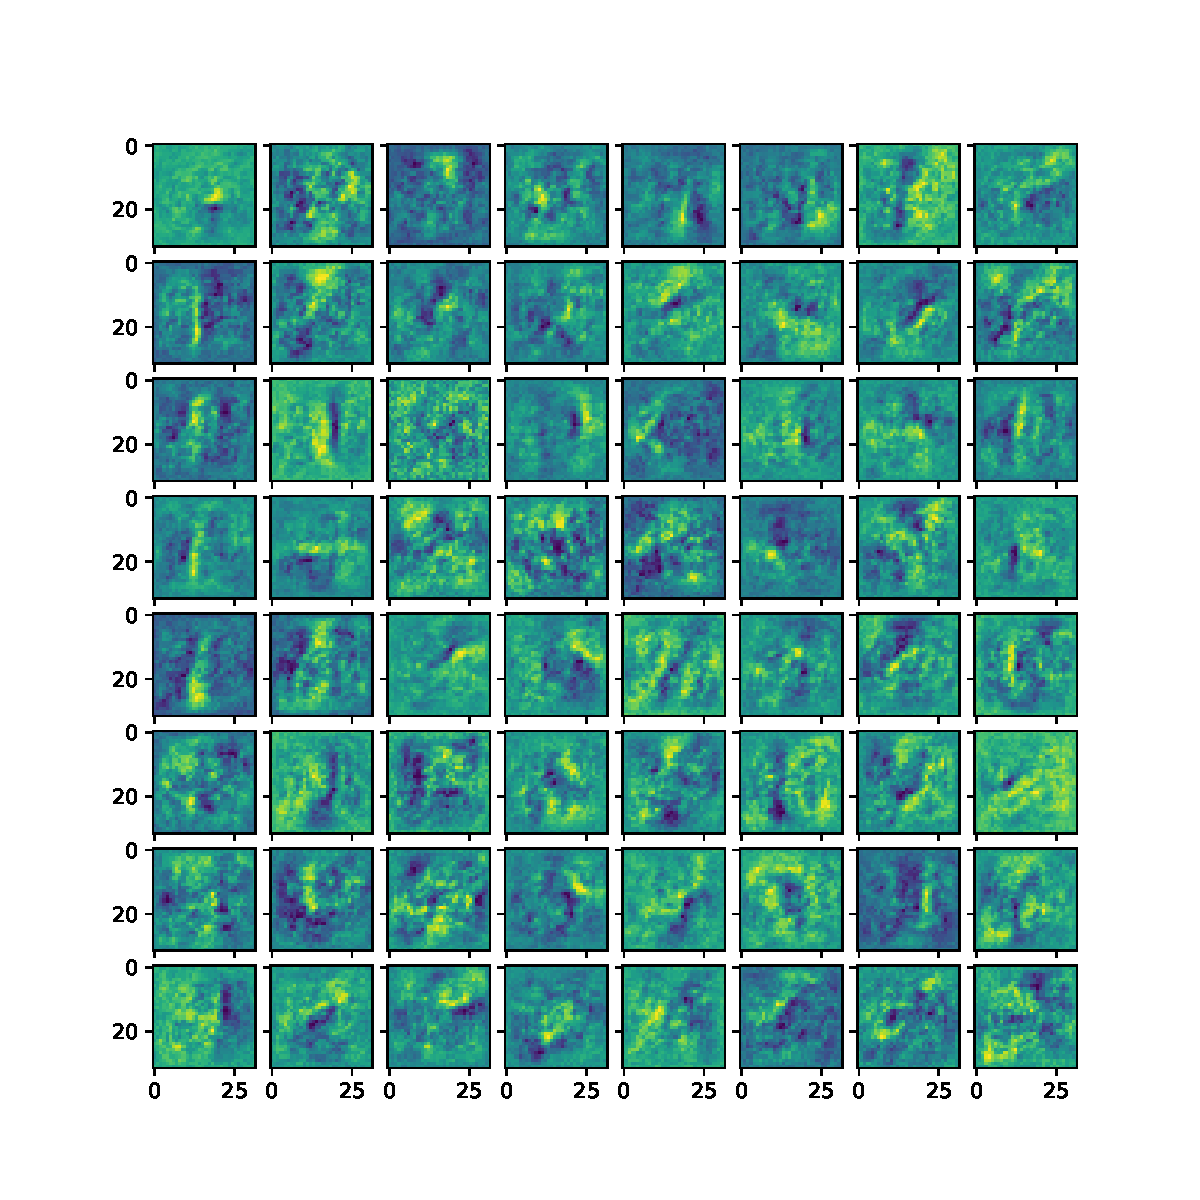
\includegraphics[width=.48\textwidth]{CV/fig/hw3/q313_1.pdf}}
    \subfigure[First Layer Weights (Before training)]{
    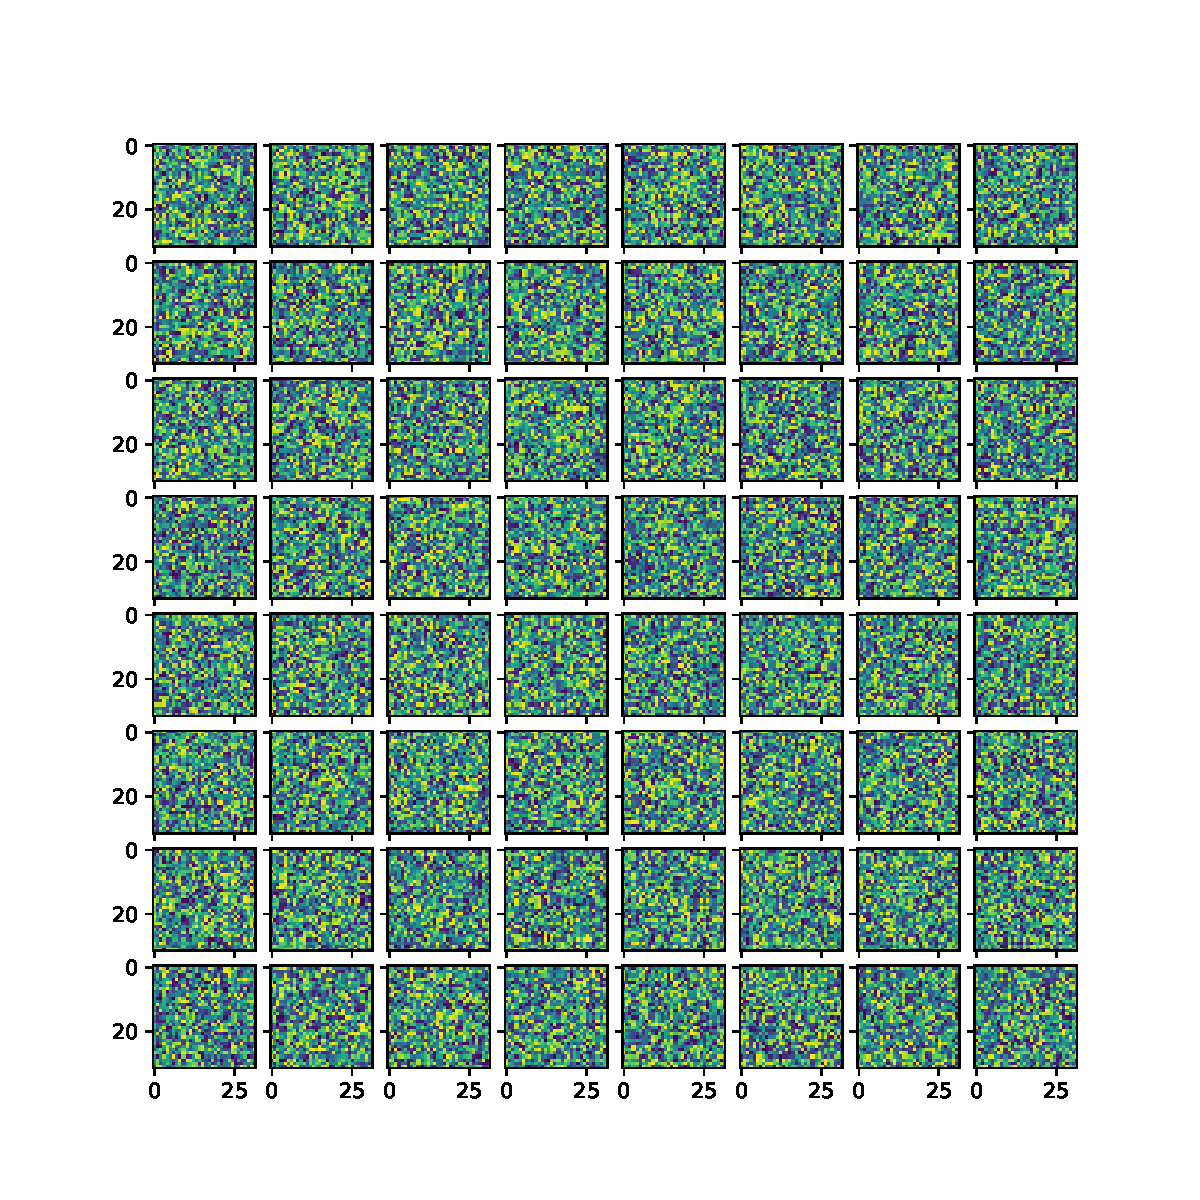
\includegraphics[width=.48\textwidth]{CV/fig/hw3/q313_2.pdf}}
    \caption{Q3.1.3}
    \label{fig:cv_hw3_q313}
\end{figure}

\noindent \textbf{Q3.1.4}

Fig. \ref{fig:cv_hw3_q314} is the result. Unlike Fig. \ref{fig:cv_hw3_q313} in Q3.1.3 just recognizing specific strokes, this activation map recognizes specific characters. We can clearly see patterns of `A', `B', `C', `G', `H', `I', `K', `N', `O', `Q', `R', `S, `X', `Z', `0',`2',`3',`8'.

\begin{figure}
    \centering
    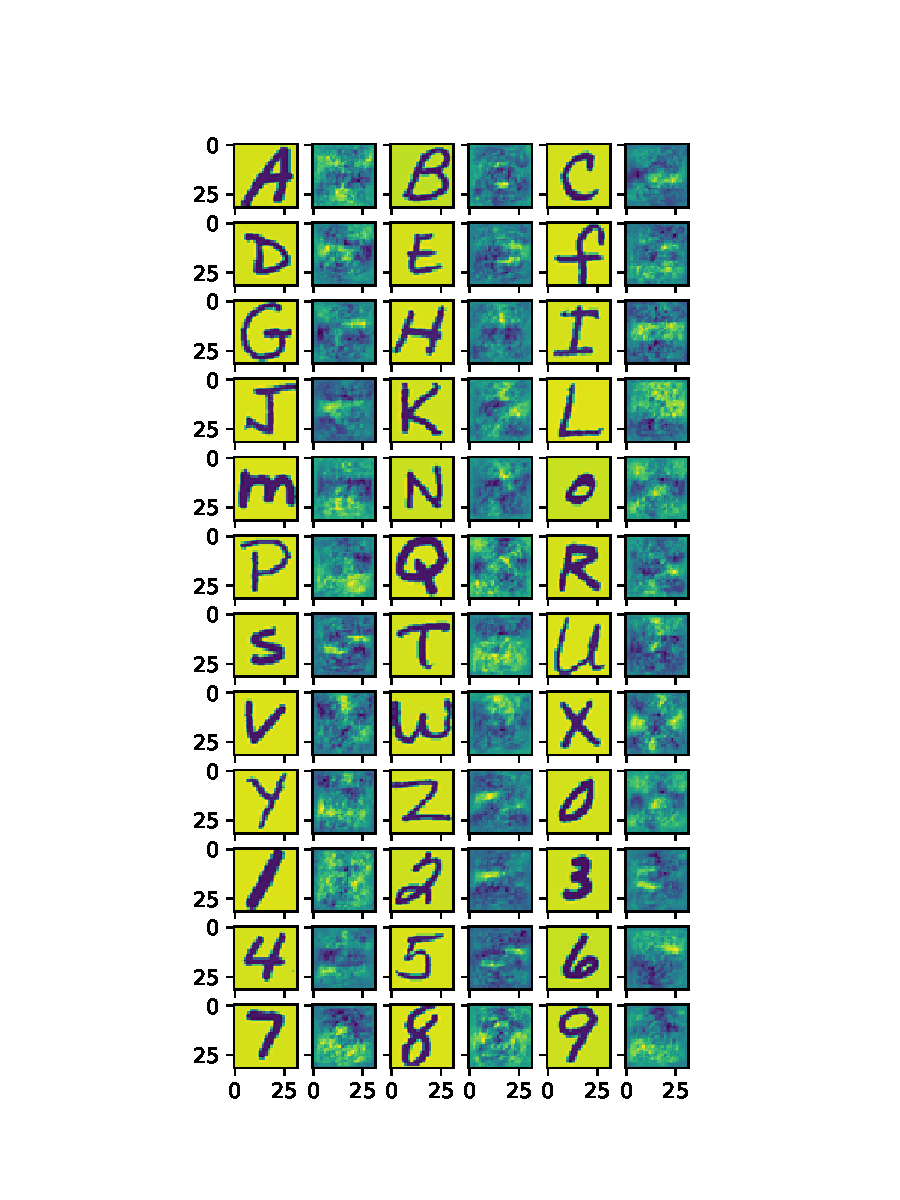
\includegraphics{CV/fig/hw3/q314.pdf}
    \caption{Q3.1.4}
    \label{fig:cv_hw3_q314}
\end{figure}

\noindent \textbf{Q3.1.5}

Fig. \ref{fig:cv_hw3_q315} is the result. The y-axis means the true label while x-axis means the predicted label. Many `O's are mislabeled as `0', and also, a few `0's are mislabeled as `O'. This is because `O' and `0' are very similar in shape. The same phenomenon also occurs for (`S', `5') and (`Z', `2') because they're similar, too. Many `H's are mislabeled as `N' because both have 2 vertical strokes on two sides. 

\begin{figure}
    \centering
    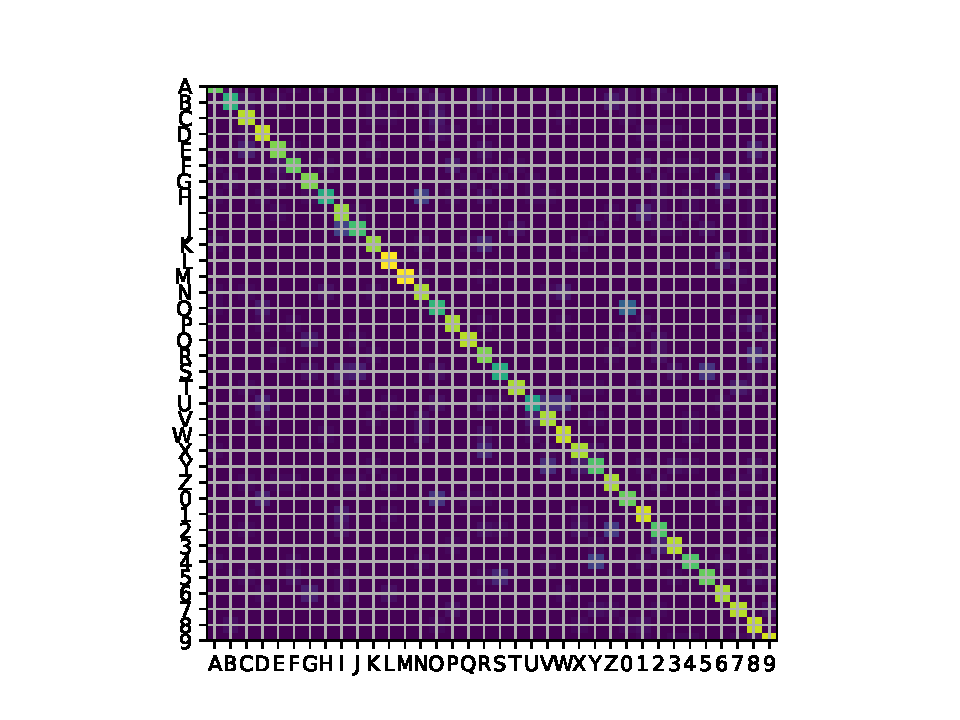
\includegraphics{CV/fig/hw3/q315.pdf}
    \caption{Q3.1.5: Confusion Matrix: y-axis means the true label while x-axis means the predicted label.}
    \label{fig:cv_hw3_q315}
\end{figure}

\section{Extract Text from Images}
\noindent\textbf{Q4.1}

The most 2 important assumptions are that ``all the pixels in one character are connected, and no pixels across different characters are connected''. The method above cannot handle self-separated characters such as `i' and `j' (Fig. \ref{fig:cv_hw3_q41_1}). Also, it cannot handle continuous writing in handwritten words (Fig. \ref{fig:cv_hw3_q41_2}).

\begin{figure}
    \centering
    \subfigure[self-separated characters]{
    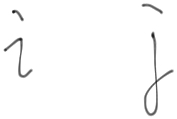
\includegraphics[width=.2\textwidth]{CV/fig/hw3/q41_1.jpeg}
    \label{fig:cv_hw3_q41_1}
    }
    \subfigure[cross-connected characters]{
    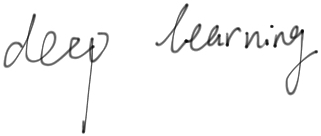
\includegraphics[width=.3\textwidth]{CV/fig/hw3/q41_2.jpeg}
    \label{fig:cv_hw3_q41_2}
    }
    \caption{Q4.1}
    \label{fig:cv_hw3_q41}
\end{figure}

\noindent \textbf{Q4.3}

Fig. \ref{fig:cv_hw3_q43} is the result.

\begin{figure}
    \centering
    \subfigure{
    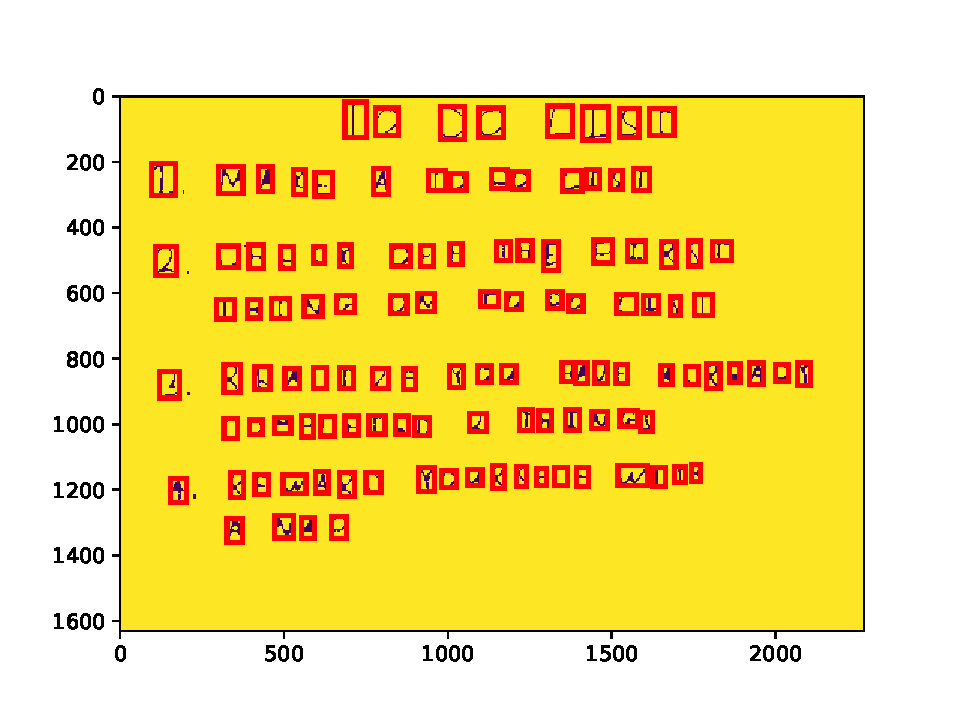
\includegraphics[width=.42\textwidth]{CV/fig/hw3/01_list.pdf}
    }
    \subfigure{
    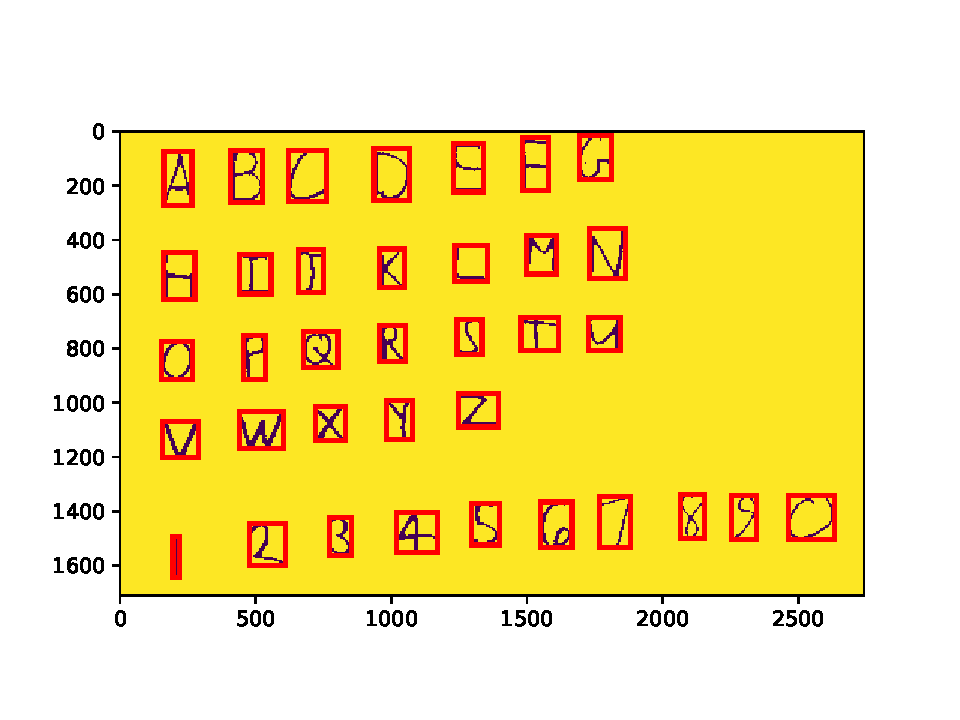
\includegraphics[width=.45\textwidth]{CV/fig/hw3/02_letters.pdf}
    }
    \subfigure{
    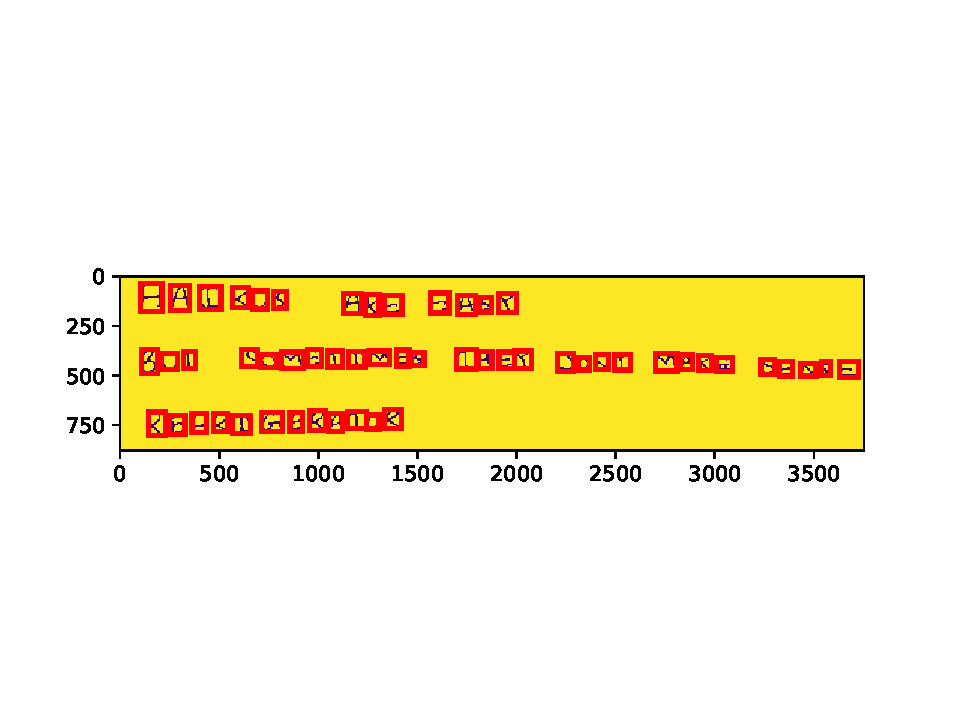
\includegraphics[width=.8\textwidth]{CV/fig/hw3/03_haiku.pdf}
    }
    \subfigure{
    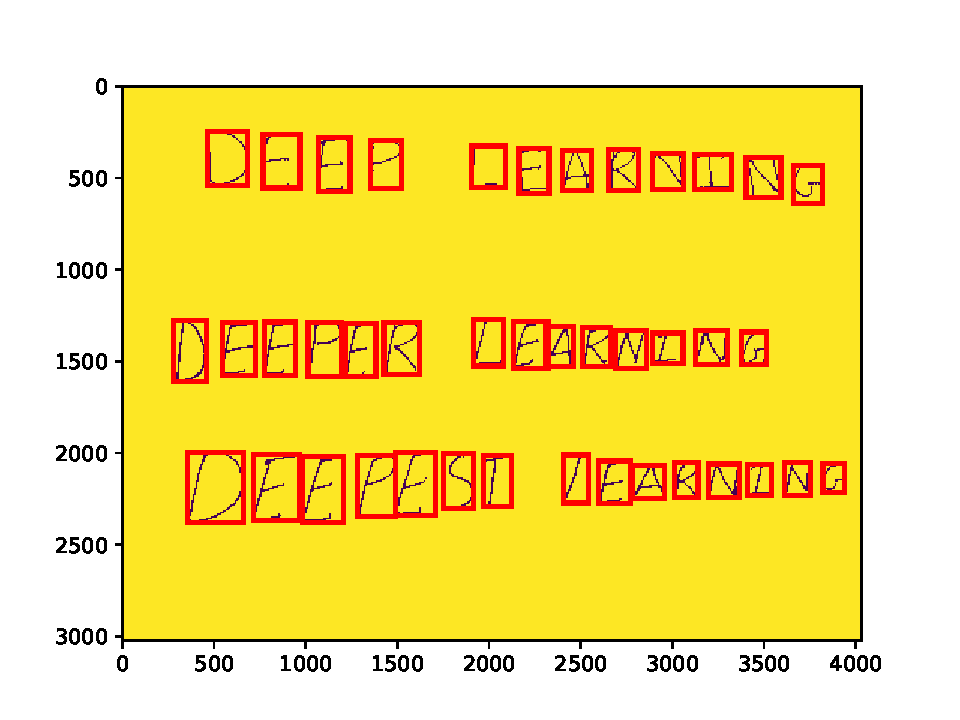
\includegraphics[width=.6\textwidth]{CV/fig/hw3/04_deep.pdf}
    }
    \caption{Q4.3}
    \label{fig:cv_hw3_q43}
\end{figure}

\noindent \textbf{Q4.4}

The overall accuracy is $80.9\%$. The extracted text are as follow (separated by lines):
\begin{itemize}
    \item \textbf{01\_list:} \\ T0 D0 LIST\\ I M2RE A TQ DQ LIST \\ 2 CHFCK QFF THE FIRST\\ THING QN TQ DQ LIIT\\ 3 R6ALIZE Y0U HAVE ALR6ADT\\ CQMPLFT6D 2 THINGI\\ 4 R8WARD Y0URSELF WITR\\ A NAP
    \item \textbf{02\_letters:} \\ ABLDEFG \\ HIJKLRN \\ QPQRSTW \\ VWX7Z \\ 1Z3GS6789Q
    \item \textbf{03\_haiku:}\\ HAIKUS ARE EAGX \\ BUT SQME TIMEG TREX DDWT MAK2 BENGE \\ RBFRIGERATQR
    \item \textbf{04\_deep:} \\ DEEP LEARMING \\ DEEPER LEARRING \\ DE8PESI LEARNING
    
\end{itemize}


\section{Image Compression with Autoencoders}
\subsection{Building the Autoencoder}
\subsection{Training the Autoencoder}
\noindent\textbf{Q5.2}

Fig. \ref{fig:cv_hw3_q52} is the training loss curve. The loss drops rapidly at the start of training, but decreases more and more slowly during the training, and finally changes little in the end of 100 epochs.

\begin{figure}
    \centering
    \subfigure{
    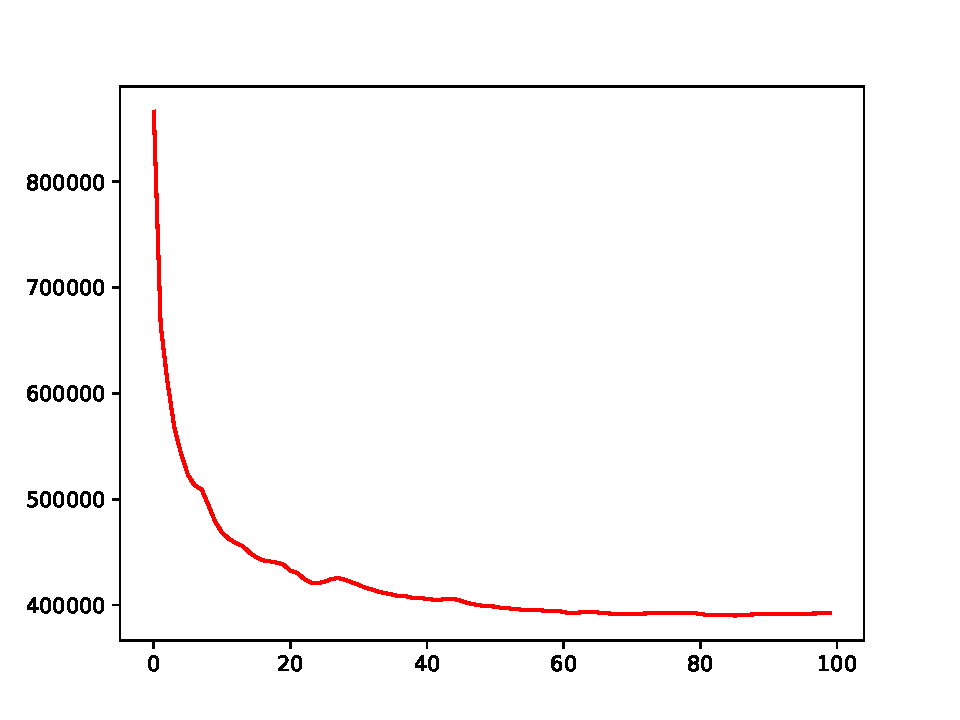
\includegraphics[width=.6\textwidth]{CV/fig/hw3/q52.pdf}}
    \caption{Q5.2: Training loss curve of the autoencoder.}
    \label{fig:cv_hw3_q52}
\end{figure}

\subsection{Evaluating the Autoencoder}
\noindent \textbf{Q5.3.1}

Fig. \ref{fig:cv_hw3_q531} is the result. I randomly pick 2 samples from each class in NIST36. The reconstructed images reserve some of the patterns, but lose many details, and thus appearing very blurred.

\begin{figure}
    \centering
    \subfigure{
    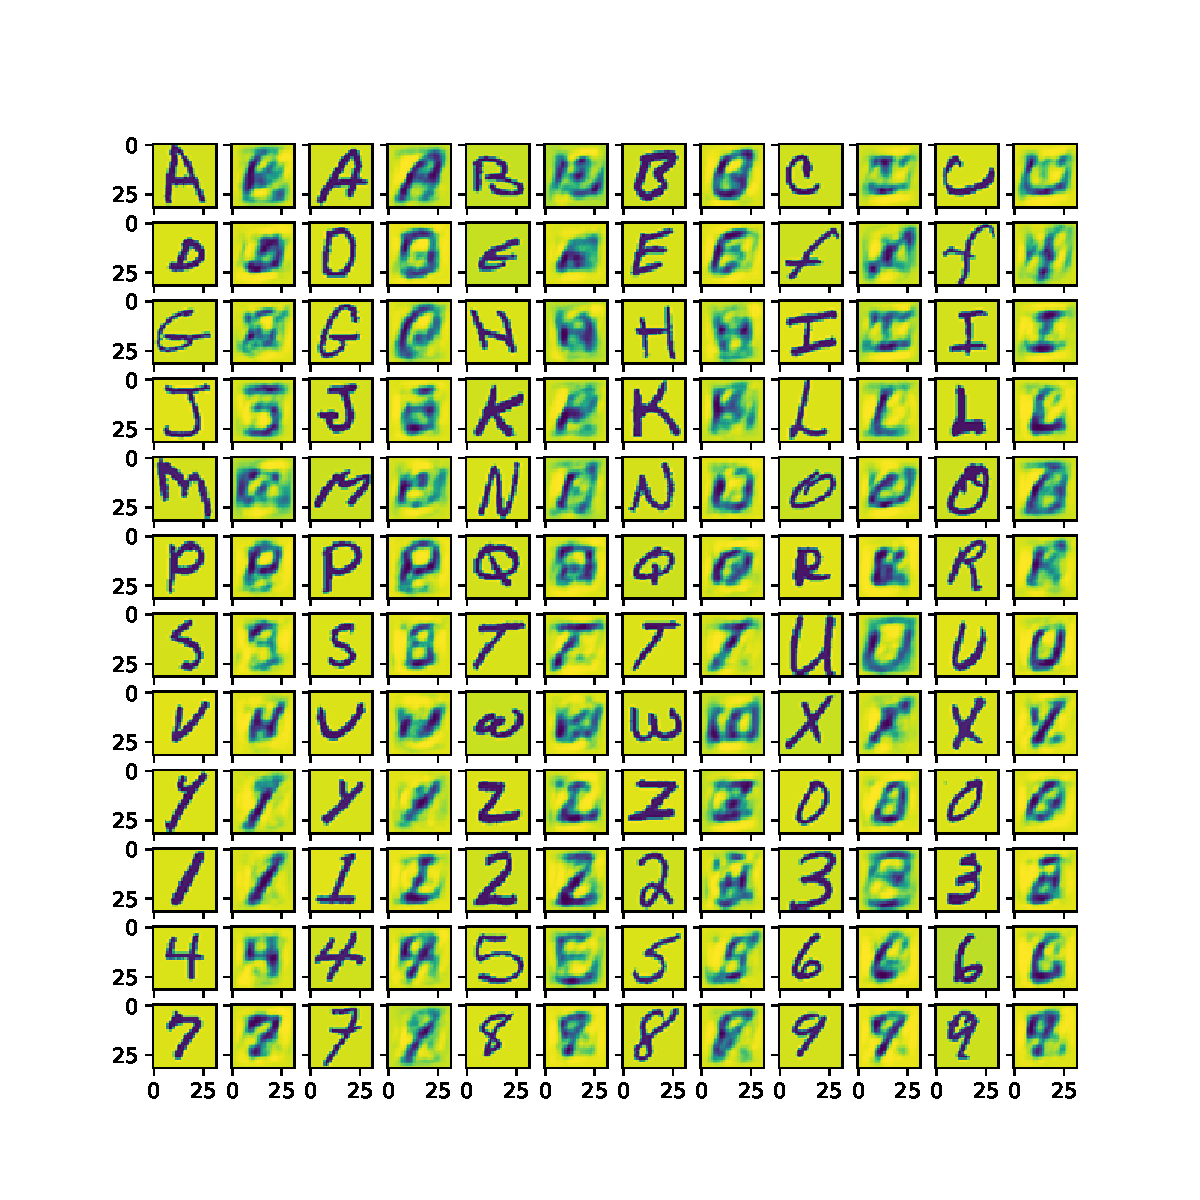
\includegraphics[width=.8\textwidth]{CV/fig/hw3/q531.pdf}}
    \caption{Q5.3.1: Result of the autoencoder.}
    \label{fig:cv_hw3_q531}
\end{figure}

\noindent \textbf{Q5.3.2}

The average PSNR across all validation images is $14.15$.

\section{Comparing against PCA}
\noindent \textbf{Q6.1}

The size of the projection matrix is $1024 \times 32$. Its rank is $32$ because its columns forms an orthonomal basis.

\noindent \textbf{Q6.2}

Fig. \ref{fig:cv_hw3_q62} is the result. Like in Q5.3.1, here I also randomly pick 2 samples from each class in NIST36. Compared with original images, those reconstructed ones have more `dirty' backgrounds, and appear a little unclear. However, PCA reconstruction performs better than the autoencoder in Q5.3.1. Strokes here are much more clear than the results of autoencoders.

\begin{figure}
    \centering
    \subfigure{
    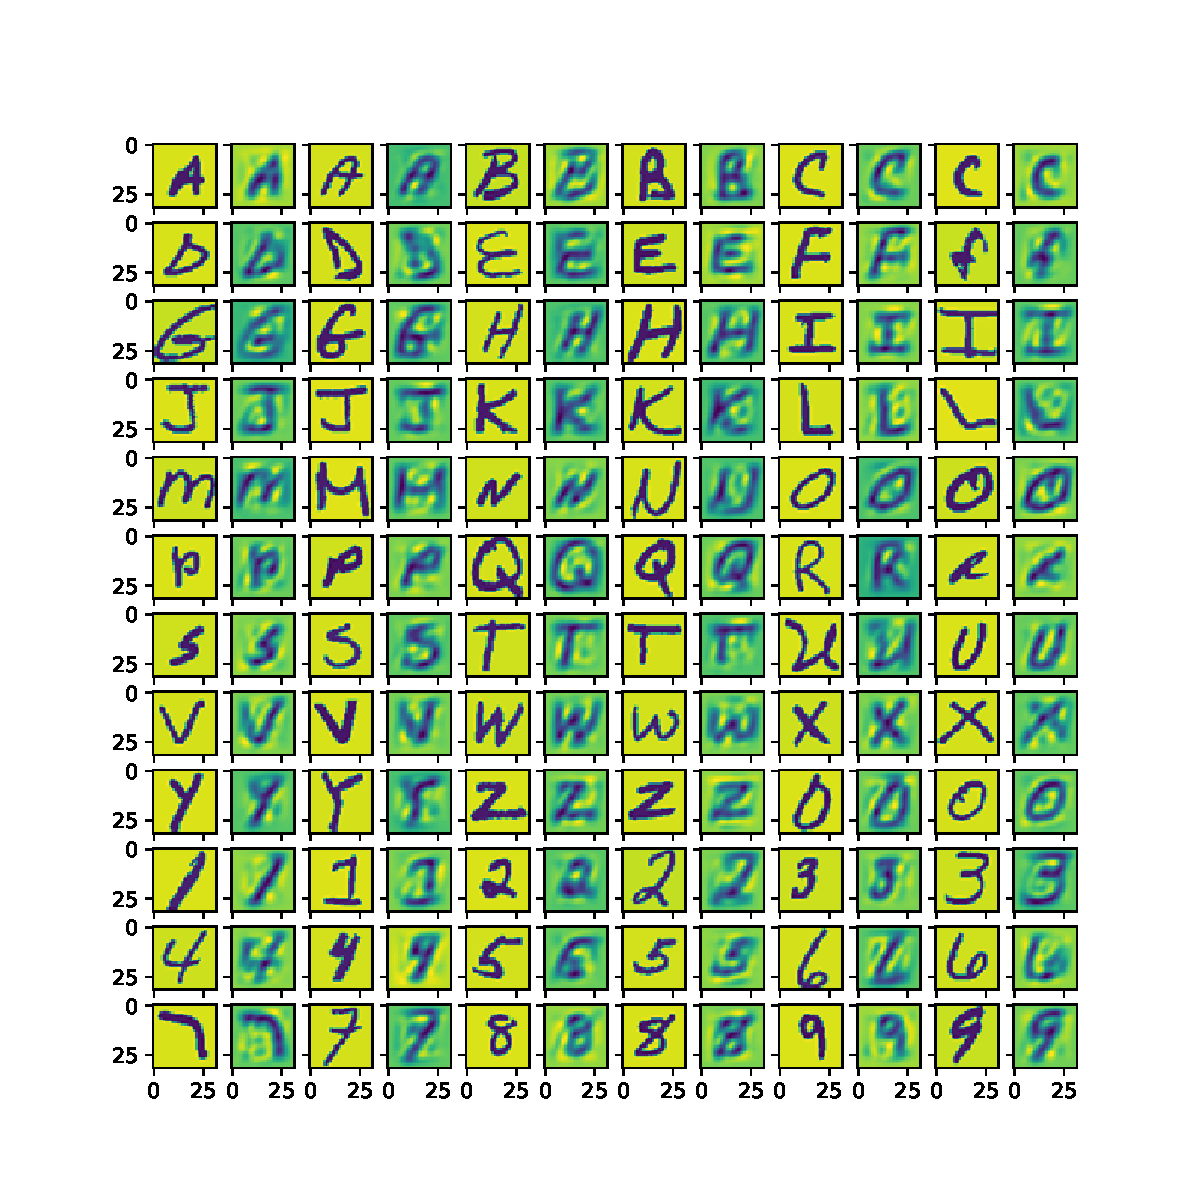
\includegraphics[width=.8\textwidth]{CV/fig/hw3/q62.pdf}}
    \caption{Q6.2: Result of PCA.}
    \label{fig:cv_hw3_q62}
\end{figure}

\noindent \textbf{Q6.3}

The average PSNR across all validation images is $16.28$, which is better than the autoencoder. Because PCA reconstructs images better than the autoencoder, so the PSNR is higher. Actually, PCA solves the best linear approximation to the training data given the reduction dim.

\noindent \textbf{Q6.4}

The PCA model has $1024 \times 32 = 32768$ parameters, while the autoencoder has $1024 \times 32 + 32 + 32 \times 32 + 32 + 32 \times 32 + 32 + 32 \times 1024 + 1024 = 67712$ parameters. PCA performs better than the autoencoder because PCA gives the exact best low-dim approximation in the linear sense, however, the neural-net autoencoder is a statistic-based method. So it does not often reaches the best solution given not so much data. Also, its optimization depends significantly on the optimization method.

\section{PyTorch}
\subsection{Train a neural network in PyTorch}
\noindent\textbf{Q7.1.1}

Fig. \ref{fig:cv_hw3_q711} is the result. I set the batch-size as $32$, and the learning rate as $5e-3$.

\begin{figure}
    \centering
    \subfigure[Accuracy]{
    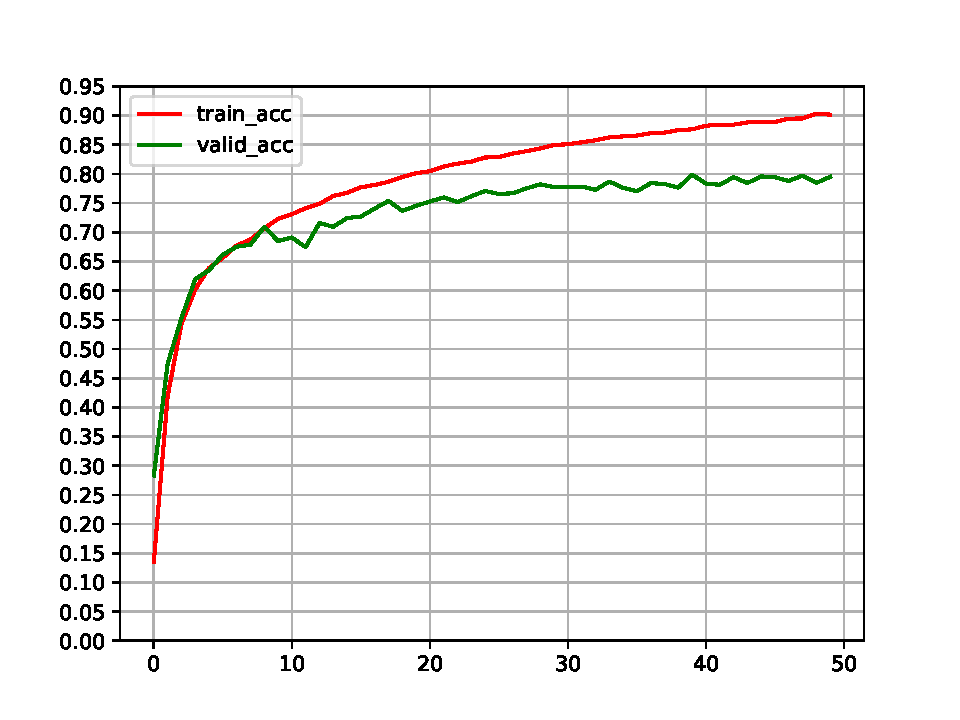
\includegraphics[width=.48\textwidth]{CV/fig/hw3/q711_acc.pdf}}
    \subfigure[Averaged Cross-Entropy Loss]{
    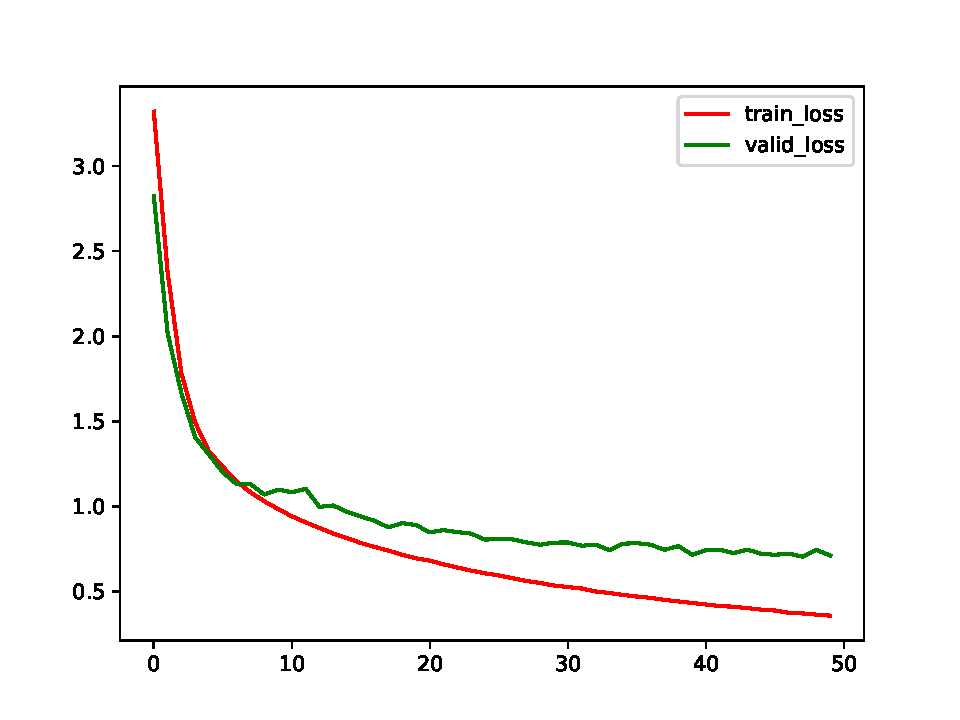
\includegraphics[width=.48\textwidth]{CV/fig/hw3/q711_loss.pdf}}
    \caption{Q7.1.1: Fully-connected network in PyTorch. lr = $5e-3$.}
    \label{fig:cv_hw3_q711}
\end{figure}

\noindent \textbf{Q7.1.2}

Fig. \ref{fig:cv_hw3_q712} is the result. I borrowed a few codes from the tutorial \url{http://cs231n.stanford.edu/notebooks/pytorch_tutorial.ipynb}.
\begin{figure}
    \centering
    \subfigure[Accuracy]{
    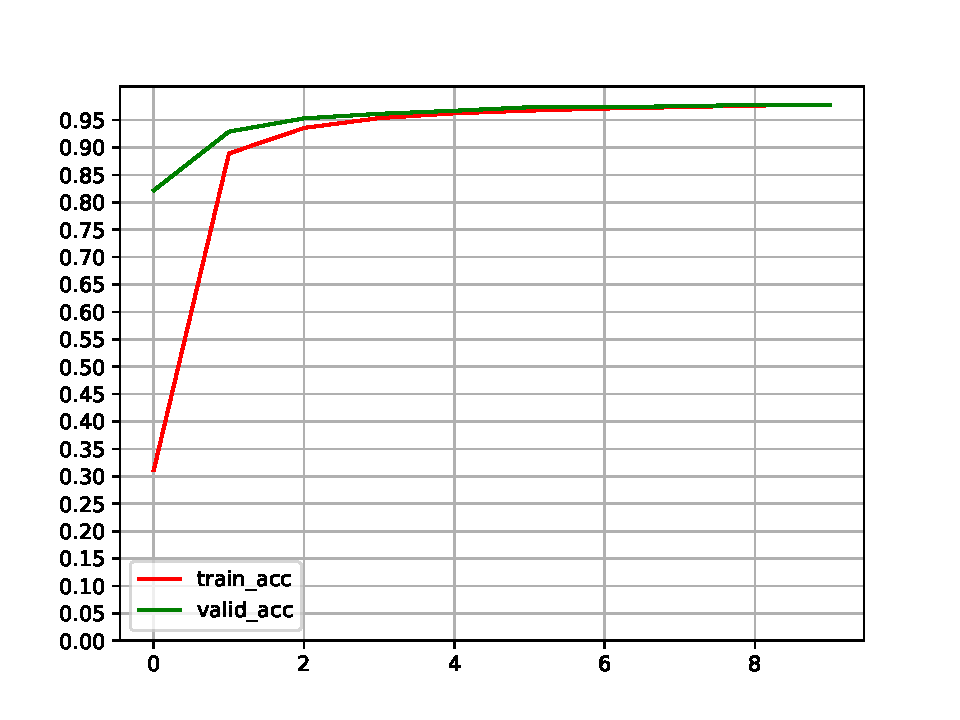
\includegraphics[width=.48\textwidth]{CV/fig/hw3/q712_acc.pdf}}
    \subfigure[Averaged Cross-Entropy Loss]{
    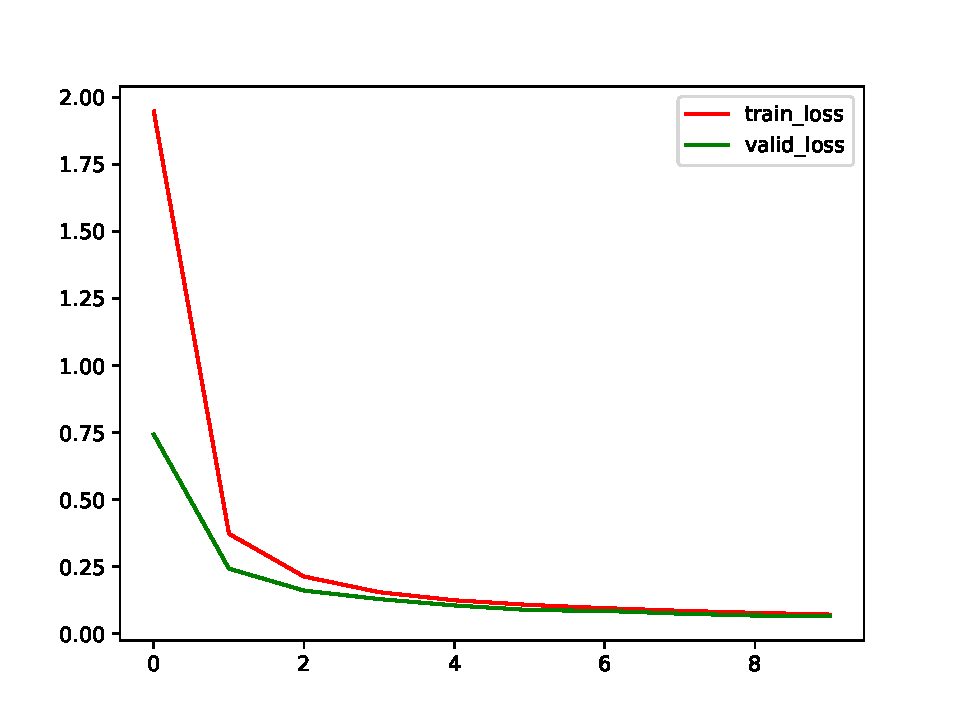
\includegraphics[width=.48\textwidth]{CV/fig/hw3/q712_loss.pdf}}
    \caption{Q7.1.2: CNN on MNIST.}
    \label{fig:cv_hw3_q712}
\end{figure}

\noindent \textbf{Q7.1.3}

Fig. \ref{fig:cv_hw3_q713} is the result. The final accuracy on the test set is $89.7\%$.

\begin{figure}
    \centering
    \subfigure[Accuracy]{
    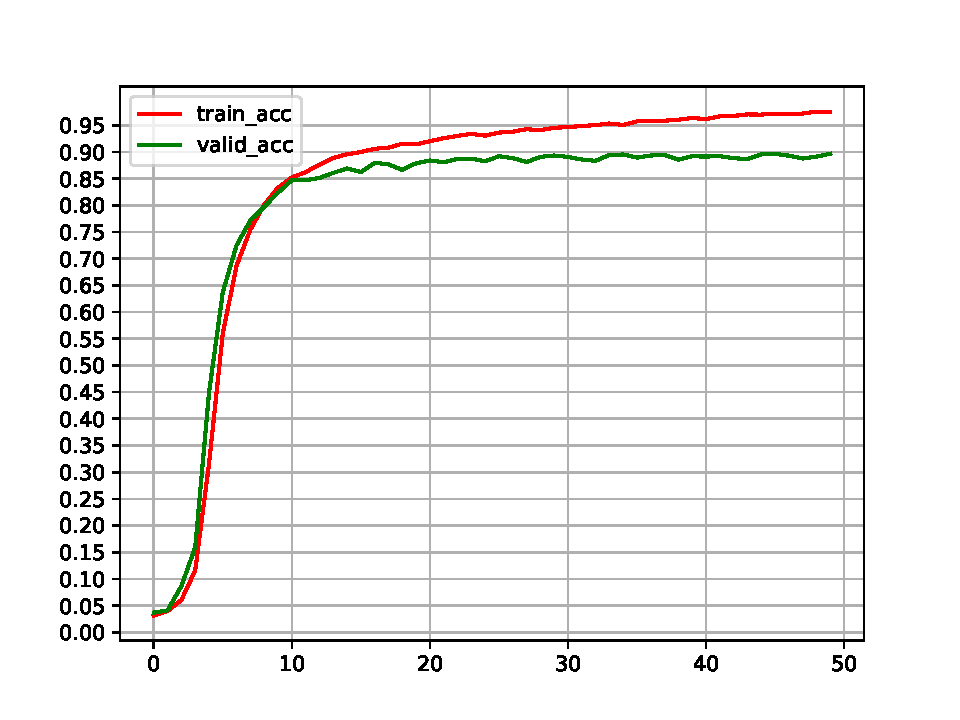
\includegraphics[width=.48\textwidth]{CV/fig/hw3/q713_acc.pdf}}
    \subfigure[Averaged Cross-Entropy Loss]{
    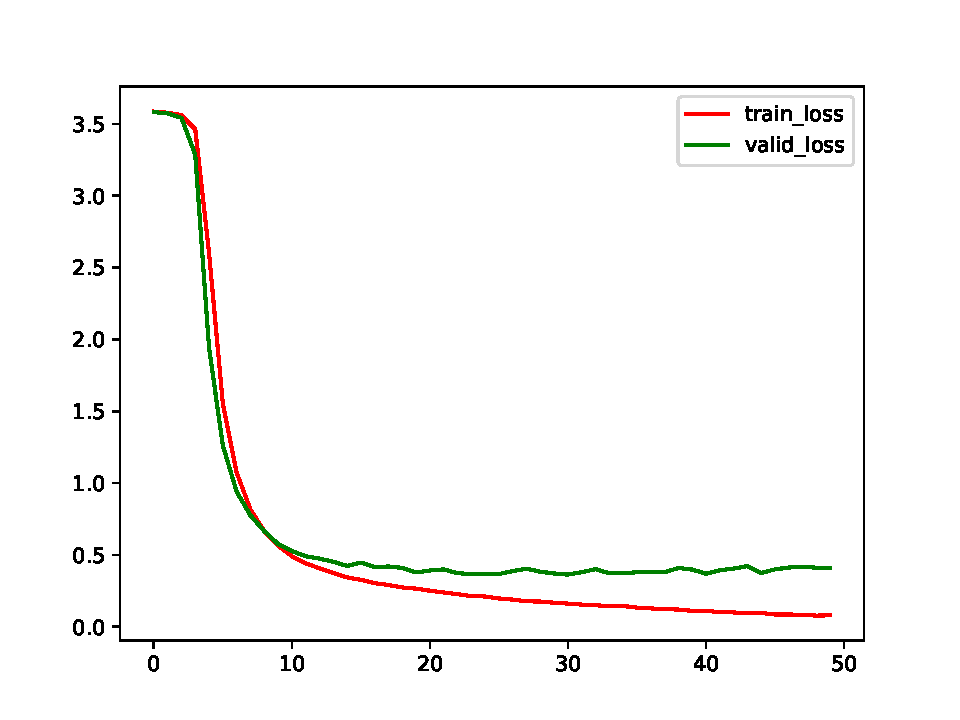
\includegraphics[width=.48\textwidth]{CV/fig/hw3/q713_loss.pdf}}
    \caption{Q7.1.3: CNN on NIST36.}
    \label{fig:cv_hw3_q713}
\end{figure}

\noindent \textbf{Q7.1.4}

The overall accuracy on the 4 test images is $63.8\%$. The extracted text are as follow:

\begin{itemize}
    \item \textbf{01\_list:} \\ 
    T0 JQ bIST \\
    i NNXR L J0 D0 LIST \\
    2 CH8CX UFF THE FIRST \\
    TBIhG 0N J0 Da CF5T\\
    3 RFaLIZE Y0U HKNE LLREADI\\
    C0MPLFYCD 2 kDPNGJ\\
    4 EFWLeU Y0URGE6F W8T4\\
    f MLP
    \item \textbf{02\_letters:} \\ gBCDEeG \\
    HIIKEYN \\
    0PQRSTW \\
    VUXfZ \\
    123aS678fO
    \item \textbf{03\_haiku:}\\ 
    HAIKUS ARE BASX\\
    BQT SOMEJIMES TXEY Q0hT MAjR SENSE\\
    RBFRIfERATDR
    \item \textbf{04\_deep:} \\ DCEP LEARNING\\DEBPER 1EARNIMG\\DFFPESe IEARWIXG
    
\end{itemize}

\subsection{Fine Tuning}
\noindent\textbf{Q7.2.1}

\noindent \textbf{Fine-tuning: } I borrow the code from the example (\url{https://gist.github.com/jcjohnson/6e41e8512c17eae5da50aebef3378a4c}), and modify it as $run\_q7\_2\_1.py$. First train the final layer for 10 epochs with the learning rate as $1e-3$, then finetune the whole model for 10 epoch with the learning rate as $1e-5$. The final accuracy on the test set is $94.4\%$.

\noindent \textbf{Scratch: } I implement a standard CNN in $run\_q7\_2\_1\_scratch.py$, and train from scratch for 50 epochs with the learning rate as $1e-3$. The final accuracy on the test set is $70.6\%$.

\noindent \textbf{Comparison: } Finetuning from a pre-trained network performs much better than training from scratch, even with less training iterations. This implies that prior knowledge in the pre-trained network plays a signicificant role in classification.

\end{document}
